% Make nice A4 pages for print:
%\usepackage{pgfpages}
%\pgfpagesuselayout{resize to}[a4paper,border shrink=5mm,landscape]

\beamertemplatenavigationsymbolsempty

\setbeamertemplate{bibliography item}[text]

\usepackage[type={CC},modifier={by-sa},version={4.0}]{doclicense}

\usepackage[utf8]{inputenc}
\usepackage{hyperref}
\usepackage{breakurl}
\usepackage{graphicx}
\usepackage{pgfplots}
\usepackage{pgf}
\usepackage{tikz}
\usetikzlibrary{positioning}
\usetikzlibrary{arrows}
\usetikzlibrary{decorations.markings}
\usetikzlibrary{calc}
\usetikzlibrary{matrix}
\usetikzlibrary{shapes}
\usetikzlibrary{decorations.pathmorphing}
\usetikzlibrary{fit}
\usetikzlibrary{backgrounds}
\usetikzlibrary{plotmarks}
\usepackage{stmaryrd}
\usepackage{listings}
\usepackage{pdflscape}
\usepackage{perpage}
\usepackage{appendixnumberbeamer}

%\usepackage[thmmarks,amsmath,amsthm]{ntheorem} % already included in beamer
\usepackage{thm-restate}

\usepackage[sort&compress,numbers]{natbib}  % to be have \citet, \citeauthor, \citeyear

\MakePerPage{footnote}

\tikzstyle{o}=[r,ppBlue]
\tikzstyle{r}=[thick,rectangle,align=center]
\tikzstyle{t}=[r,ppTrans] %,font=\bfseries]
\tikzstyle{dd}=[densely dashed]
\tikzstyle{n}=[r,ppBlue]
\tikzstyle{p}=[r,ppRed]
\tikzstyle{ppRed}  =[draw=red,  fill=  red!20]
\tikzstyle{ppBlue} =[draw=blue, fill= blue!20]
\tikzstyle{ppGreen}=[draw=green,fill=green!20]
\tikzstyle{ppTrans}=[draw=none, fill=none]

\usetheme{Warsaw}

\useoutertheme[subsection=true]{smoothbars}
%\useoutertheme[subsection=false]{miniframes}

\definecolor{bblue}{HTML}{D7DF01}	% yellow-ish actually, for better black/white printing
\definecolor{rred}{HTML}{C0504D}
\definecolor{ggreen}{HTML}{9BBB59}
\definecolor{ppurple}{HTML}{9F4C7C}
\definecolor{lightgray}{rgb}{0.3,0.3,0.3}
\definecolor{lightergray}{rgb}{0.9,0.9,0.9}
\definecolor{UniBlue}{RGB}{83,121,170}

\DeclareTextFontCommand\textintro{\normalfont\bfseries\itshape} % nice!
\newcommand{\intro}[2][]
{%
	\textintro{#2}%
}
\newcommand{\empha}[2][]
{%
	\emph{#2}%
}

%\theoremstyle{plain}
\newcounter{reqcounter}
\newtheorem{requirement}[reqcounter]{Requirement}

%setbeamercolor{structure}{fg=violet}

\makeatletter
\def\th@task{%
    \normalfont % body font
    \setbeamercolor{block title example}{bg=orange,fg=white}
    \setbeamercolor{block body example}{bg=orange!20,fg=black}
    \def\inserttheoremblockenv{exampleblock}
  }
\makeatother

\theoremstyle{task}
\newtheorem{task}{Task}

\newenvironment{assignment}%
{%\setbeamercolor{background canvas}{bg=violet}%
%\setbeamercolor{structure}{fg=cyan!90!black}%
 \setbeamercolor{frametitle}{bg=orange,fg=white}
\begin{frame}}%
{\end{frame}}%

\AtBeginSection[]{
  \begin{frame}
  \vfill
  \centering
  \begin{beamercolorbox}[sep=8pt,center,shadow=true,rounded=true]{title}
    \usebeamerfont{title}\insertsectionhead\par%
  \end{beamercolorbox}
  \tableofcontents
  \vfill
  \end{frame}
}




\pgfplotsset{compat=1.14}
\author{Markus Raab}


\date{13.3.2018}

\begin{document}

\renewcommand{\enquote}[1]{\emph{``#1''}} % Cannot be done earlier

%%%%%%%%%%%%%%%%%%%%%%%%%%%%%%%
\begin{frame}
	\titlepage
	\doclicenseThis
\end{frame}

\begin{assignment}
	\frametitle{Language of the Talk?}
	\begin{task}
	Hands up if you prefer German.
	\end{task}
\end{assignment}

\begin{frame}
	Lecture is every week Wednesday 09:00 - 11:00.

	\begin{description}
		\item[06.03.2019:] topic, teams
		\item[{\color{red}13.03.2019:}] {\color{red}TISS registration, initial PR}
		\item[20.03.2019:] other registrations, Guest Lecture
		\item[27.03.2019:] (HS?)
		\item[03.04.2019:]
		\item[08.05.2019:] (HS?)
		\item[10.04.2019:] mid-term submission of exercises
		\item[15.05.2019:]
		\item[22.05.2019:]
		\item[29.05.2019:]
		\item[05.06.2019:] final submission of exercises
		\item[12.06.2019:]
		\item[19.06.2019:] last corrections of exercises
		\item[26.06.2019:] exam
	\end{description}
\end{frame}

\begin{frame}
	\frametitle{Popular Topics}
	\vspace{-0.55cm}
	\setlength{\columnsep}{-1.3cm}
	\raggedright
	\begin{multicols}{2}
	\begin{description}
	\item[14] tools
	\item[9] testability
	\item[9] code-generation
	\item[7] context-awareness
	\item[6] specification
	\item[6] misconfiguration
	\item[6] complexity reduction
	\item[5] validation
	\item[5] points in time % (early detection)
	\item[5] error messages
	\item[5] auto-detection
	\item[4] user interface
	\item[4] introspection
	\item[4] design
	\item[4] cascading
	\item[4] architecture of access
	\item[3] {\color{red} configuration sources}
	\item[3] config-less systems
	\item[2] secure conf
	\item[2] architectural decisions
	\item[1] push vs.\ pull
	\item[1] infrastructure as code
	\item[1] full vs.\ partial
	\item[1] convention over conf %iguration
	\item[1] CI/CD
	\item[0] documentation
	\end{description}
	\end{multicols}
\end{frame}

\begin{frame}
	\frametitle{Organisation}
	\begin{itemize}
	\item https://github.com/orgs/ElektraInitiative/teams/cm2019s now created
	\item private repo created
	\item first PRs created and accepted:
	\begin{itemize}
	\item release notes often not updated
	\item please set ``ready to merge'' if build server is happy
	\end{itemize}
	\end{itemize}
\end{frame}

\begin{frame}
	\frametitle{Talk}
	about anything related to configuration management.
	\begin{itemize}
		\item The duration \textbf{must be not longer} than 20 minutes (shorter is ok, content matters).
		\item It must be about your experience.
		\begin{itemize}
			\item E.g., about the homework you did.
			\item I.e., not only about study of literature.
			\item If you extensively use some tool before, please share your experience.
		\end{itemize}
		\item Two persons per date.
		\item Same topic allowed if persons coordinate their talk.
	\end{itemize}
\end{frame}

\begin{assignment}
	\frametitle{Next tasks}
	\begin{task}
	Initial PR must be done \textbf{today}, can be trivial
	\end{task}

	\begin{task}
	Registration for talk, homework, teamwork until 20.03.2019 23:59
	\end{task}

	\begin{task}
	Assign yourself at least one issue or ask me to assign one to you.
	(make sure to say which programming languages you know)
       	Deadline: 20.03.2019 23:59
	\end{task}
\end{assignment}

\begin{frame}
	\textit{learning outcome:}
	\begin{itemize}
		\item Having an overview of configuration file formats.
		\item Understanding Elektra's abstractions that deals with the multitude of configuration file formats.
	\end{itemize}
\end{frame}



\section{Configuration File Formats}

\subsection{Definitions}

\begin{frame}
	\frametitle{Basic Definitions}
	The \intro[execution environment]{execution environment} is information outside the boundaries of each currently running process~\cite{corbato1971multics}.

	Controlling the execution environment is essential for configuration management~\cite{cons2002pan,huang2015confvalley}, testing~\cite{van2010automating,wang2009context}, and security~\cite{goldberg1996secure,schreuders2012towards,perkins2009automatically,liang2003isolated}.
\end{frame}

\begin{frame}
	\frametitle{Configuration Setting}
	\begin{definition}
\label{def:configuration-setting}
A \intro[configuration setting]{configuration setting},
or \intro[setting|see{configuration setting}]{setting} in short,
fulfills these properties:
\begin{enumerate}
\item
It is provided by the execution environment.
\item
It is \empha[consume]{consumed} by an application.
\item
It consists of a key, a configuration value, and potentially \empha{metadata}.
The \intro{configuration value}, or \intro[value|see{configuration value}]{value} in short, influences the application's behavior.
\item
It can be \empha[produce]{produced} by the maintainer, user, or system administrator of the software.
\end{enumerate}
\end{definition}

\end{frame}


\begin{frame}[fragile]
	\frametitle{Synonyms for Configuration Settings}
	\ExecuteMetaData[../book/background.tex]{synonyms}
\end{frame}

\begin{frame}[fragile]
	\frametitle{Definition}
	A \intro{configuration file} is a file containing configuration settings.

	\pause
	A Web server configuration file:

	\begin{lstlisting}[gobble=4]
	port=80 ; comment
	address=127.0.0.1\end{lstlisting}

	\only<2-2>{
	\begin{task}
	What are keys? What are configuration values? What is metadata?
	\end{task}
	}
	\pause

	The configuration values are ^80^ and ^127.0.0.1^, respectively.
	Other information in the configuration file is metadata for the configuration settings (such as the comment).
\end{frame}

\subsection{Formats}

\begin{frame}
	\frametitle{Types of Formats}
	\begin{itemize}
	\item CSV (comma-separated values)
	\item semi-structured
	\item programming language
	\item document-oriented
	\item literate
	\end{itemize}
\end{frame}

\begin{frame}
	\frametitle{CSV formats}
	\begin{itemize}
	\item passwd: \formatdate{3}{11}{1971}
	\item passwd and group use : as separator
	\item are difficult to extend (e.g., GECOS)
	\item today mostly used for legacy reasons
	\item are replaced one-by-one (e.g., inetd, crontab)
	\end{itemize}
\end{frame}

\begin{frame}
	\frametitle{Trends}
	\begin{itemize}
	\item away from CSV
	\item towards general-purpose serialization formats (INI, JSON)
	\item human-read/writable (YAML, HOCON, TOML)
	\item programming language as configuration file
	\end{itemize}
\end{frame}

\begin{frame}
	\frametitle{Programming Language}
	\begin{description}
	\item[$+$] very easy for developers (simply source the file)
	\item[$+$] above-overage quality of error message
	\item[$-$] makes automatic change of individual values harder
	\item[$-$] very hard to use for people who do not know the programming language
	\item[$-$] does not separate code and data
	\end{description}
\end{frame}

\begin{assignment}
	\frametitle{Introduce somebody}
	\begin{task}
	Talk with someone about your favourite configuration file format.
	\end{task}

	\begin{task}
	Did you implement a configuration file parser and/or invented a new configuration file format?
	\end{task}

	\begin{task}
	Explain to everyone about the other person and his/her favourite configuration file format.
	\end{task}
\end{assignment}

\begin{frame}
	\frametitle{Method}

	What do FLOSS developers say?

	\begin{description}
	\item[\methodQuestion{}] survey with 672 persons visiting, 162 persons completing the survey~\cite{raab2017challenges}
	\item[\methodSource{}] source code analysis of 16 applications, comprising 50 million lines of code~\cite{raab2017challenges}
	\end{description}
\end{frame}

\begin{frame}
	\frametitle{Why are so many formats present?}
	\methodQuestion{} \question{In which way have you used or contributed to the configuration system/library/API in your previously mentioned FLOSS project(s)?}~\cite{raab2017challenges}
	\begin{itemize}
	\item \p{19} persons ($n=251$) have introduced a configuration file format.
	\item \p{29} implemented a configuration file parser.
	\item \p{15} introduced a configuration system/library/API.
	\item \p{34} used external configuration access APIs.
	\end{itemize}
\end{frame}

\begin{frame}
	\frametitle{Multitude of Formats}
	\begin{itemize}
	\item on every system a multitude of (legacy) configuration file formats exist
	\item the number grows fast
	\item thus applications usually have to deal with some legacy formats
	\end{itemize}
	

	\begin{restatable}{requirement}{reqLegacy}
	A configuration library must be able to integrate (legacy) systems and must fully support (legacy) configuration files.%
	\label{req:legacy}
	\end{restatable}
\end{frame}


%%%%%%%%%%%%%%%%%%%%%%%%%%%%%%%%%%%%%%%%%% 
\section{Elektra}

\subsection{Basics}

\begin{frame}
	\frametitle{Elektra as Virtual Filesystem}
	\begin{itemize}
	\item configuration files are seen like ``block devices''
	\item are mounted with respective filesystem drivers into the filesystem
	\item many tools and APIs evolved to work with files
	\item Idea of Elektra: establish a similar ecosystem for configuration
	\end{itemize}
\end{frame}

\begin{frame}
	\frametitle{Why is Elektra not a Filesystem then?}
	\begin{itemize}
	\item API semantics: key/value get/set
	\item namespaces: based on established semantics
	\item many features essential for misconfiguration hardening:
		\begin{itemize}
		\item validation
		\item visibility
		\item defaults
		\item \dots (extensible specification)
		\end{itemize}
	\end{itemize}
\end{frame}

% hack: needed to render graphics properly
\begin{frame}<0>[noframenumbering]
	\begin{columns}[c]
	\begin{column}{7cm}
	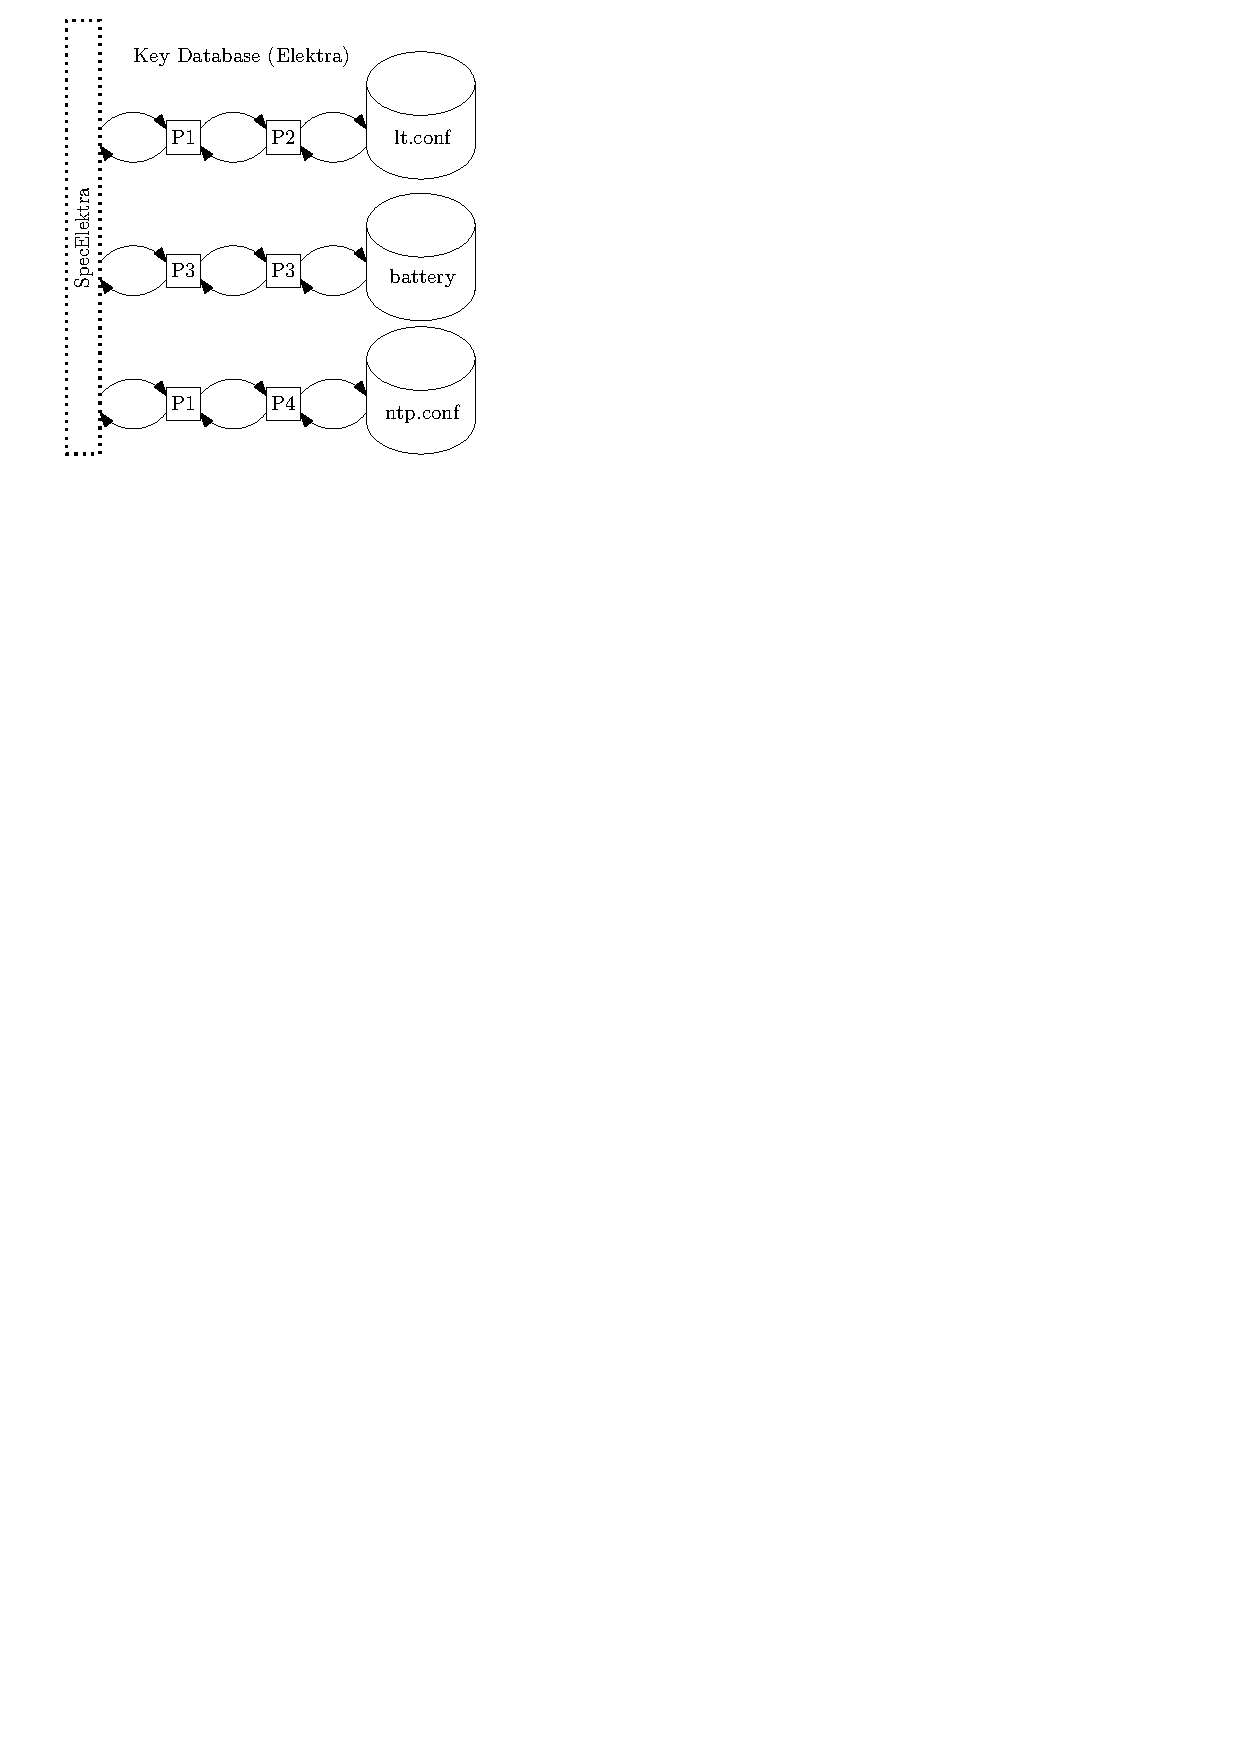
\includegraphics[scale=0.8]{horizontalmodularity}
	\end{column}
	\begin{column}{4cm}
	Cylinders are configuration files, P? are plugins~\cite{raab2016improving}.

	Key ideas:
	\begin{itemize}
	\item all work is done by plugins
	\item central data structure implements semantics
	\end{itemize}
	\end{column}
	\end{columns}
\end{frame}

\begin{frame}
	\begin{columns}[c]
	\begin{column}{7cm}
	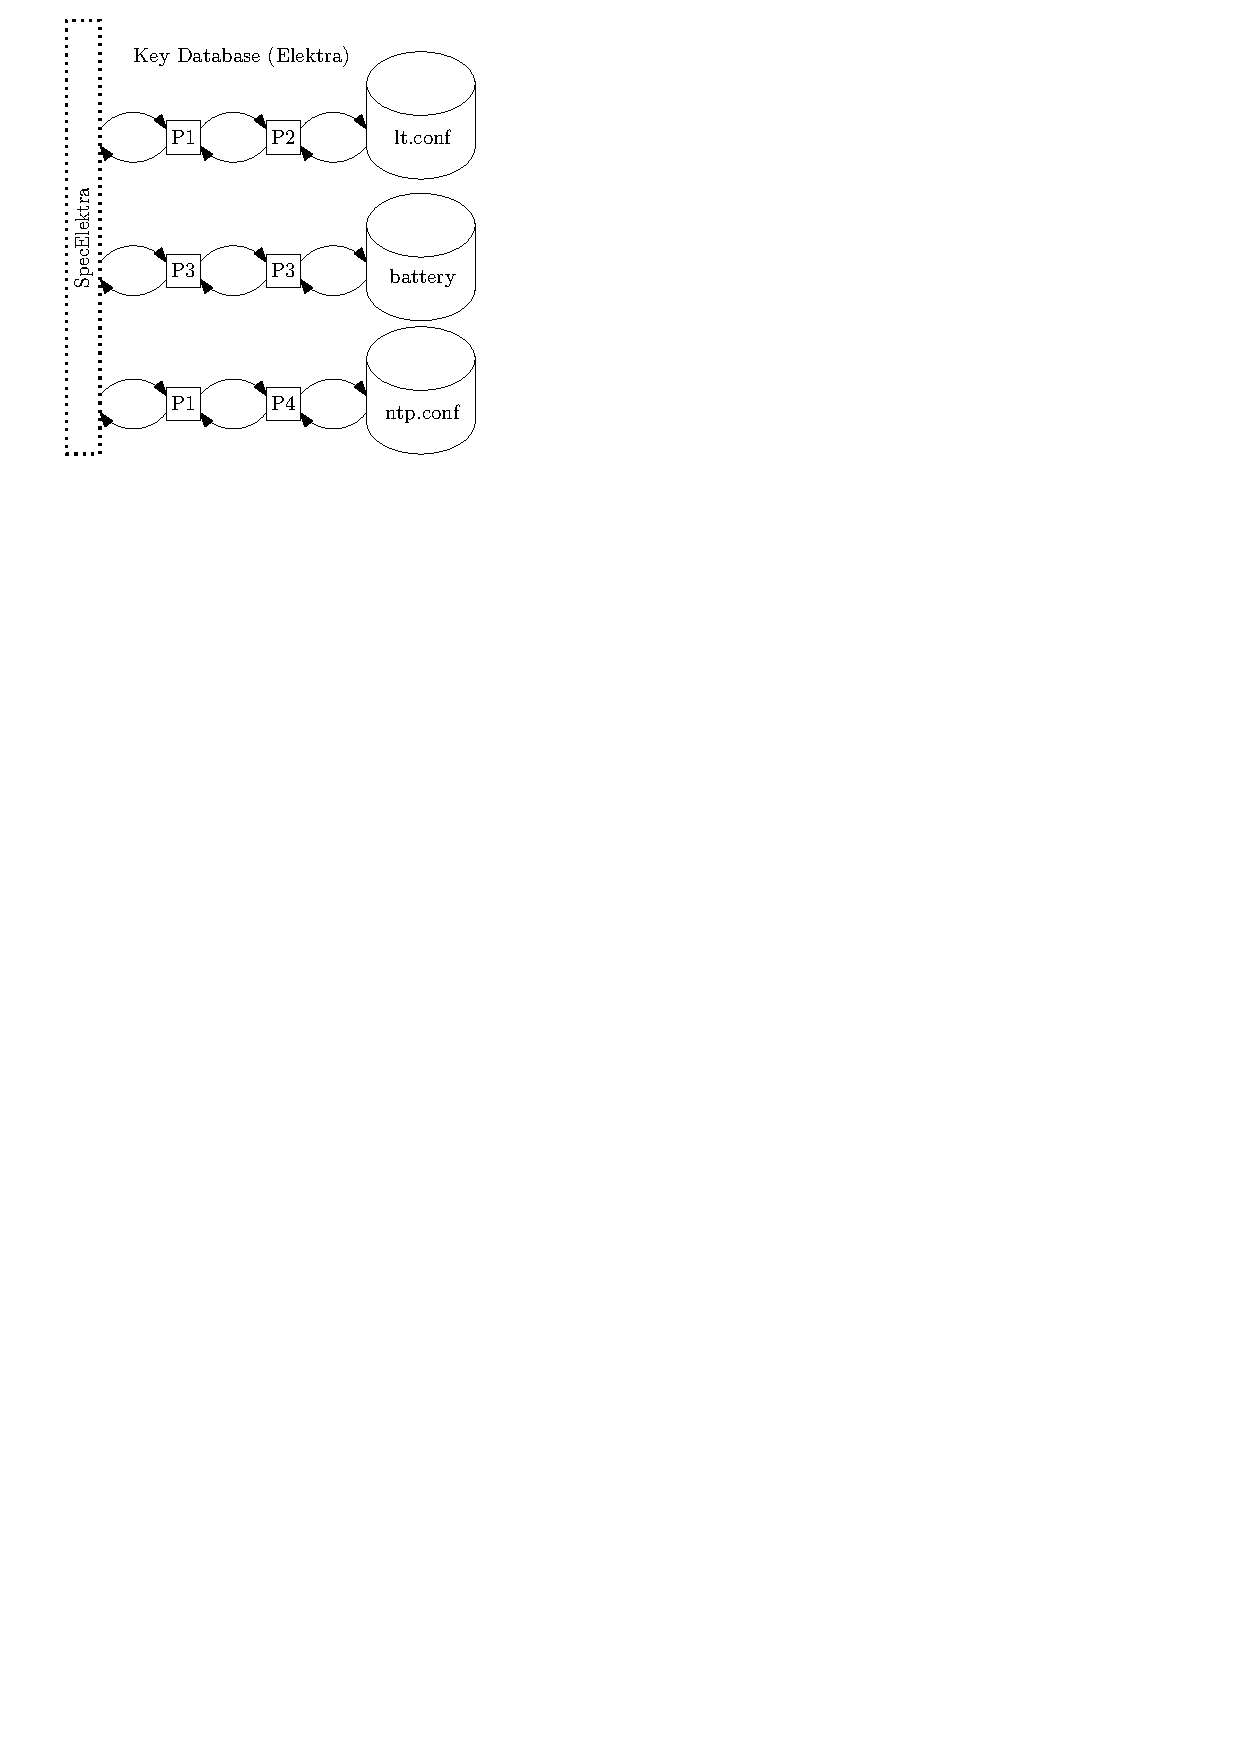
\includegraphics[scale=0.8]{horizontalmodularity}
	\end{column}
	\begin{column}{4cm}
	Cylinders are configuration files, P? are plugins~\cite{raab2016improving}.

	Key ideas:
	\begin{itemize}
	\item all work is done by plugins
	\item central data structure implements semantics
	\end{itemize}
	\end{column}
	\end{columns}
\end{frame}

\begin{frame}
	\frametitle{KeySet}

	The common data structure between plugins:
	\vspace{1cm}

	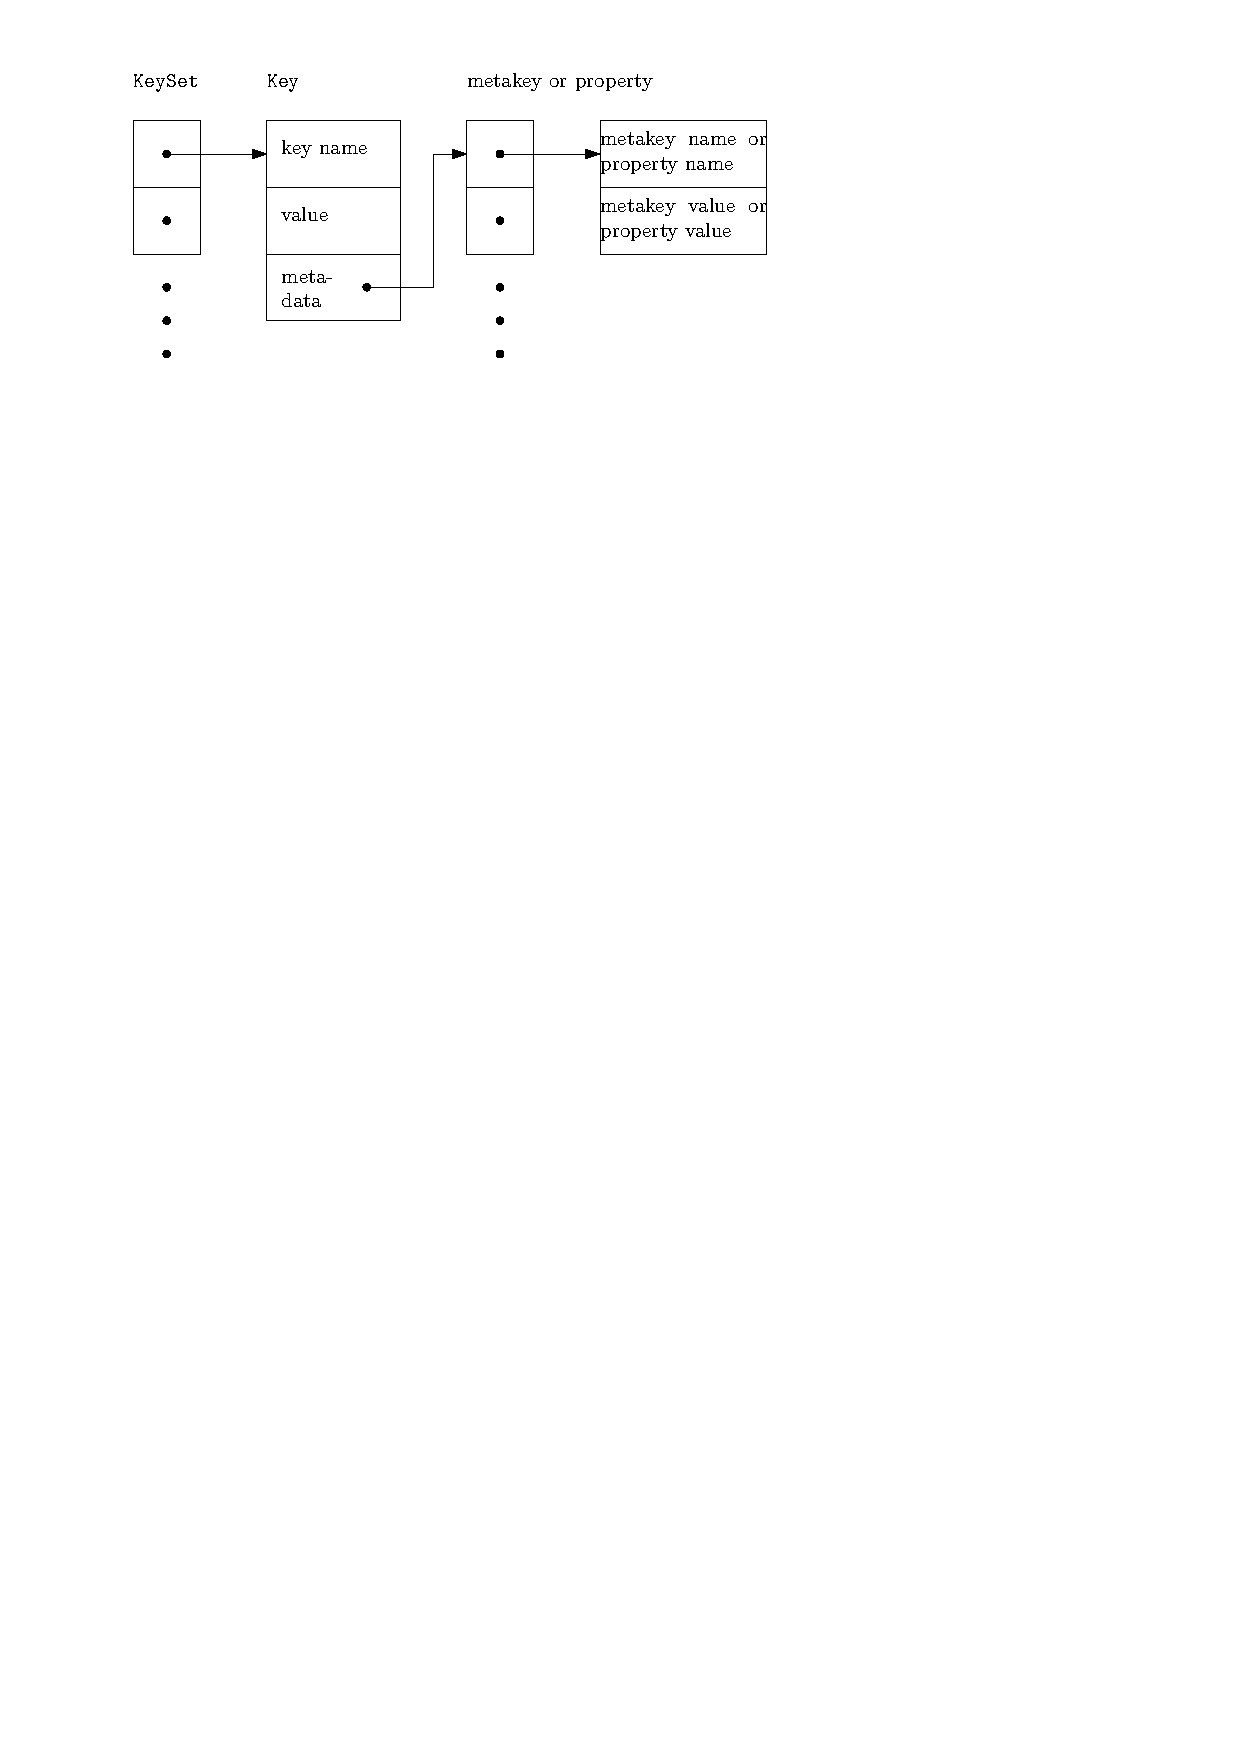
\includegraphics{keyset}
\end{frame}

\begin{assignment}
	\begin{task}
	Is meta-data separated from or included in the data structure?
	\end{task}
\end{assignment}

\begin{frame}[fragile]
	\begin{description}[align=left]
	\item[kdb.open():]
	The first step is to bootstrap into a situation where the necessary plugins can be loaded.
	\item[kdb.get(\texttt{KeySet}):] \index{kdb.get}
	The application (initially) fetches and (later) updates its configuration settings as a key set of type ^KeySet^ from the execution environment by one or many calls to ^kdb.get^.
	%If all relevant configuration files are unmodified since the last invocation, ^kdb.get^ will do nothing.
	\item[kdb.set(\texttt{KeySet}):] \index{kdb.set}
	When a user finishes editing configuration settings, ^kdb.set^ is in charge of writing all changes back to the key database.
	%This function atomically persists a whole key set in involved parts of the execution environment.
	%In the case of an error no action takes place.
	\item[kdb.close():] \index{kdb.close}
	The last step is to close the connection to the key database.
	\end{description}
\end{frame}

\begin{assignment}
	\begin{task}
	Break.
	\end{task}
\end{assignment}

\subsection{Metalevels}

\begin{frame}
	\frametitle{Metalevels}
	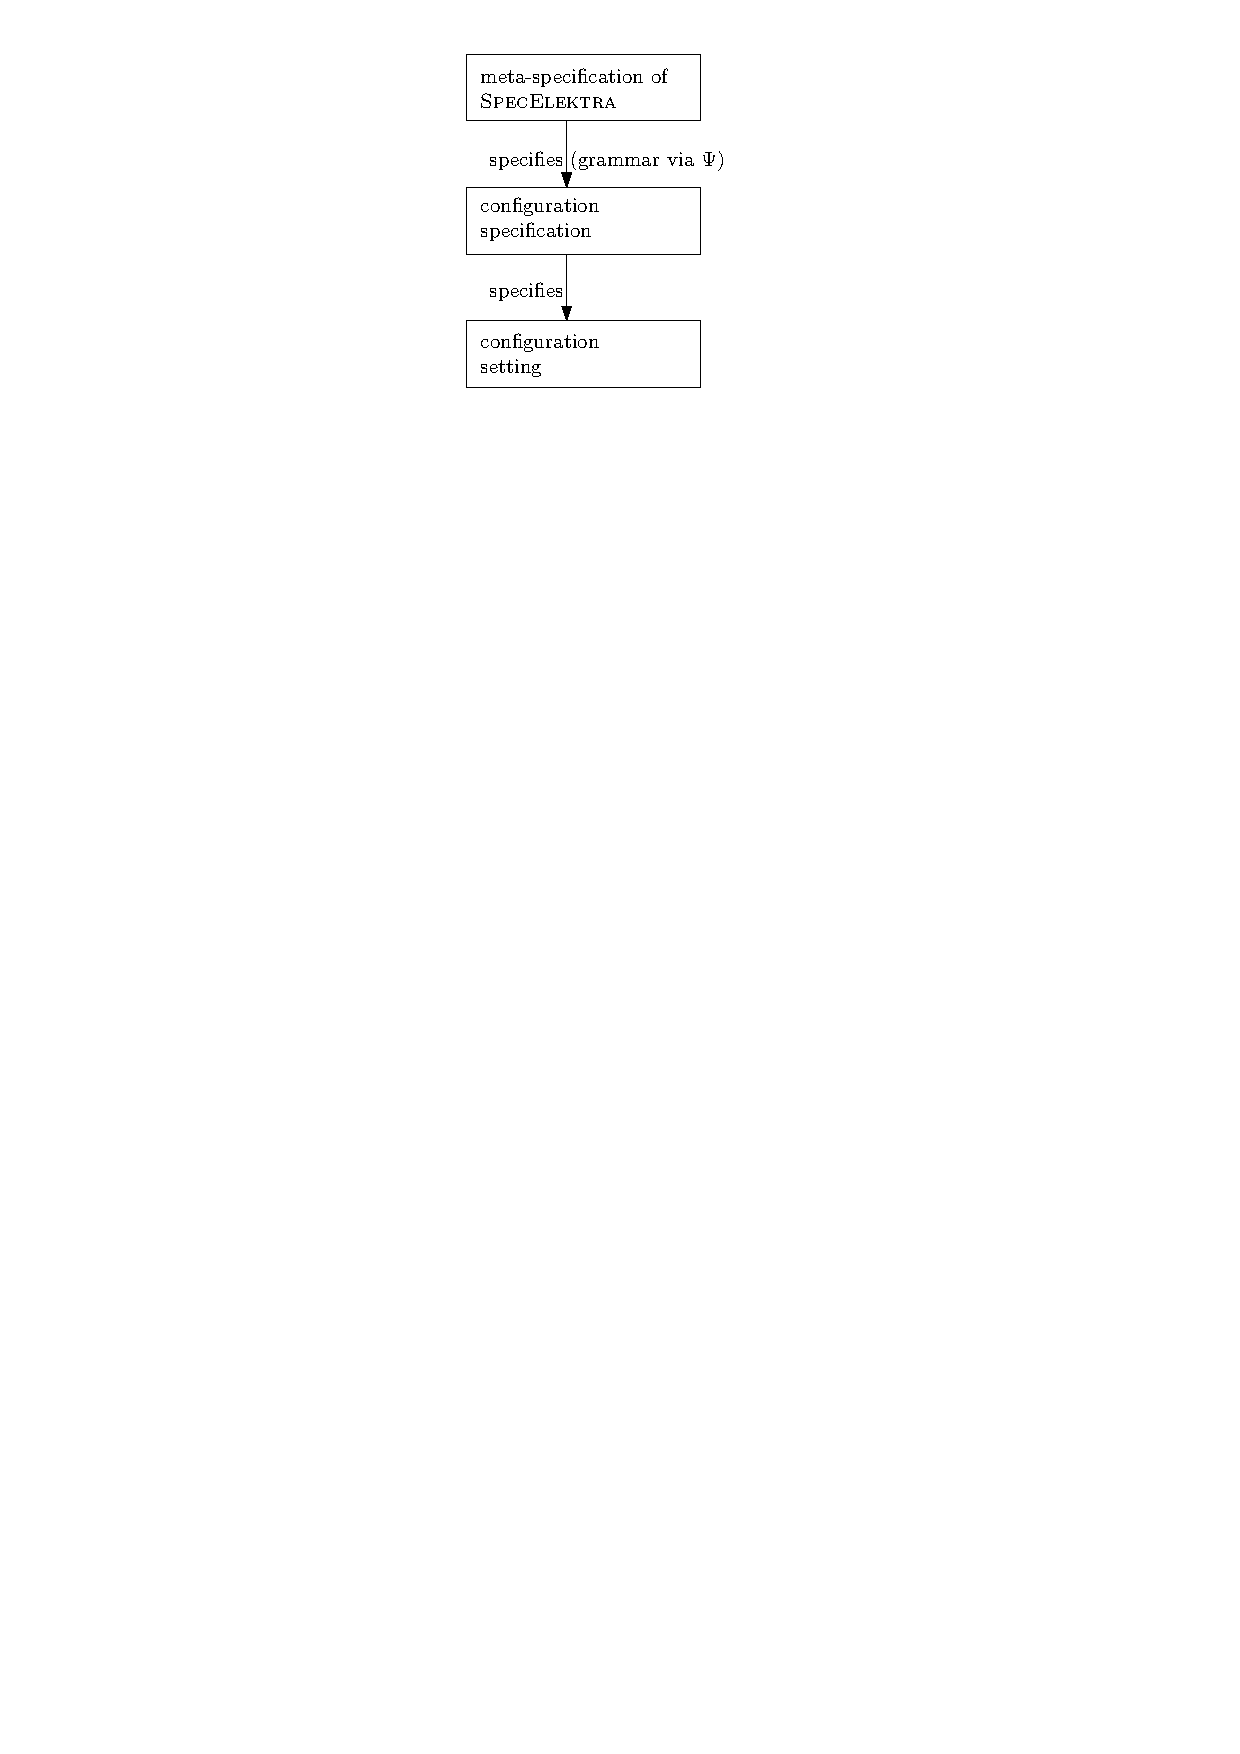
\includegraphics{metalevels}

	We will now walk through metalevels bottom-up.
\end{frame}

\begin{frame}[fragile]
	\frametitle{Configuration Settings}

	A configuration file may look like:

	\begin{code}[language=CfgElektra]
	a=5
	b=10
	c=15
	\end{code}

	We apply these configuration settings imperatively using:

	\begin{code}[language=bash]
	kdb set /a 5
	kdb set /b 10
	kdb set /c 15
	\end{code}

	And we list them with \lstinline[language=bash,morekeywords={ls},showspaces=no]^kdb ls /^.
\end{frame}

\begin{frame}[fragile]
	\frametitle{Specifications}
	For specifications such as:

	\begin{code}
	[slapd/threads/listener]
	  check/range:=1,2,4,8,16
	  default:=1
	\end{code}

	We apply the specifications imperatively using:

	\begin{code}[language=bash,morekeywords={setmeta}]
	kdb setmeta /slapd/threads/listener\
		check/range 1,2,4,8,16
	kdb setmeta /slapd/threads/listener\
	       	default 1
	\end{code}

	(automatically uses ^spec^ namespace)
\end{frame}

\begin{frame}[fragile]
	\frametitle{Meta-Specifications}
	For meta-specifications such as:

	\small
	\begin{code}
	[visibility]
	type:=enum critical important user\
	      advanced developer debug disabled
	description:=Who should see this\
	     configuration setting?
	\end{code}

	We apply the meta-specifications imperatively using:

	\begin{code}[language=bash,morekeywords={setmeta}]
	kdb setmeta /elektra/meta/\
		visibility type enum ...
	kdb setmeta /elektra/meta/\
		visibility description "Who ...
	\end{code}

	(see ^doc/METADATA.ini^, disclaimer: 1.0 not yet released)
\end{frame}

\begin{assignment}
	\begin{task}
	Brainstorming: Ideas for (meta-)specifications.
	\end{task}
\end{assignment}

\subsection{Conclusions}

\begin{frame}
	\frametitle{Introspection}
	\begin{itemize}[<+->]
	\item unified get/set access to (meta*)-key/values
	\item access via applications, CLI, GUI, web-UI, ...
	\item GUI, web-UI can semantically interpret metadata
	\item access via any programming language
	\item access via any configuration management system
	\end{itemize}
\end{frame}

\begin{frame}
	\frametitle{Users of Elektra}
	\begin{itemize}[<+->]
	\item Embedded systems
	\begin{itemize}
	\item OpenWRT (distribution)
	\item Broadcom (blue-ray devices)
	\item Kapsch (cameras)
	\item Toshiba (TVs)
	\end{itemize}
	\item Server
	\begin{itemize}
	\item Allianz (insurance)
	\item TU Wien
	\item puppet-libelektra
	\item Other Universities
	\end{itemize}
	\item Desktop
	\begin{itemize}
	\item Oyranos
	\item LCDproc (in progress)
	\item KDE
	\end{itemize}
	\end{itemize}
\end{frame}

\begin{frame}
	\frametitle{Conclusion}
	\begin{itemize}
	\item goals:
		\begin{itemize}
		\item make simple configuration management tasks simple
		\item improve robustness
		\item improve extensibility (reusable plugins operating on key/value)
		\item improve performance
		\item good defaults
		\item system-wide introspection
		\item system-level dependency injection
		\end{itemize}
	\item \elektra{} has no dependence to other libraries but only concrete plugins introduce dependences.
	\end{itemize}
\end{frame}



%%%%%%%%%%%%%%%%%%%%%%%%%%%%%%%%%%%%%%%%%%%%%%%%%%%%
\section{Abstractions}

\subsection{Mounting}

\begin{frame}
	\frametitle{Abstraction}
	\reqLegacy*

	\vspace{1cm}

	How can we deal with the many formats?
\end{frame}


\begin{frame}
	\frametitle{Key-Value}
A key-value pair is the simplest generic data structure~\cite{strang2004context}.
While all these formats above have many differences, all of them represent configuration settings as \intro[key-value pair]{key-value pairs}~\cite{jin2014configurations,rabkin2011static,xu2013blame,lathia2013open}.
\\[1cm]

For configuration as program you need to execute them first.
\end{frame}

\begin{frame}
	\frametitle{Mounting}
	\intro[mounting]{Mounting} integrates a backend into the key database~\cite{raab2008thesis}.
	Hence, \elektra{} allows several backends to deal with configuration files at the same time.
	Each backend is responsible for its own subtree of the key database.

	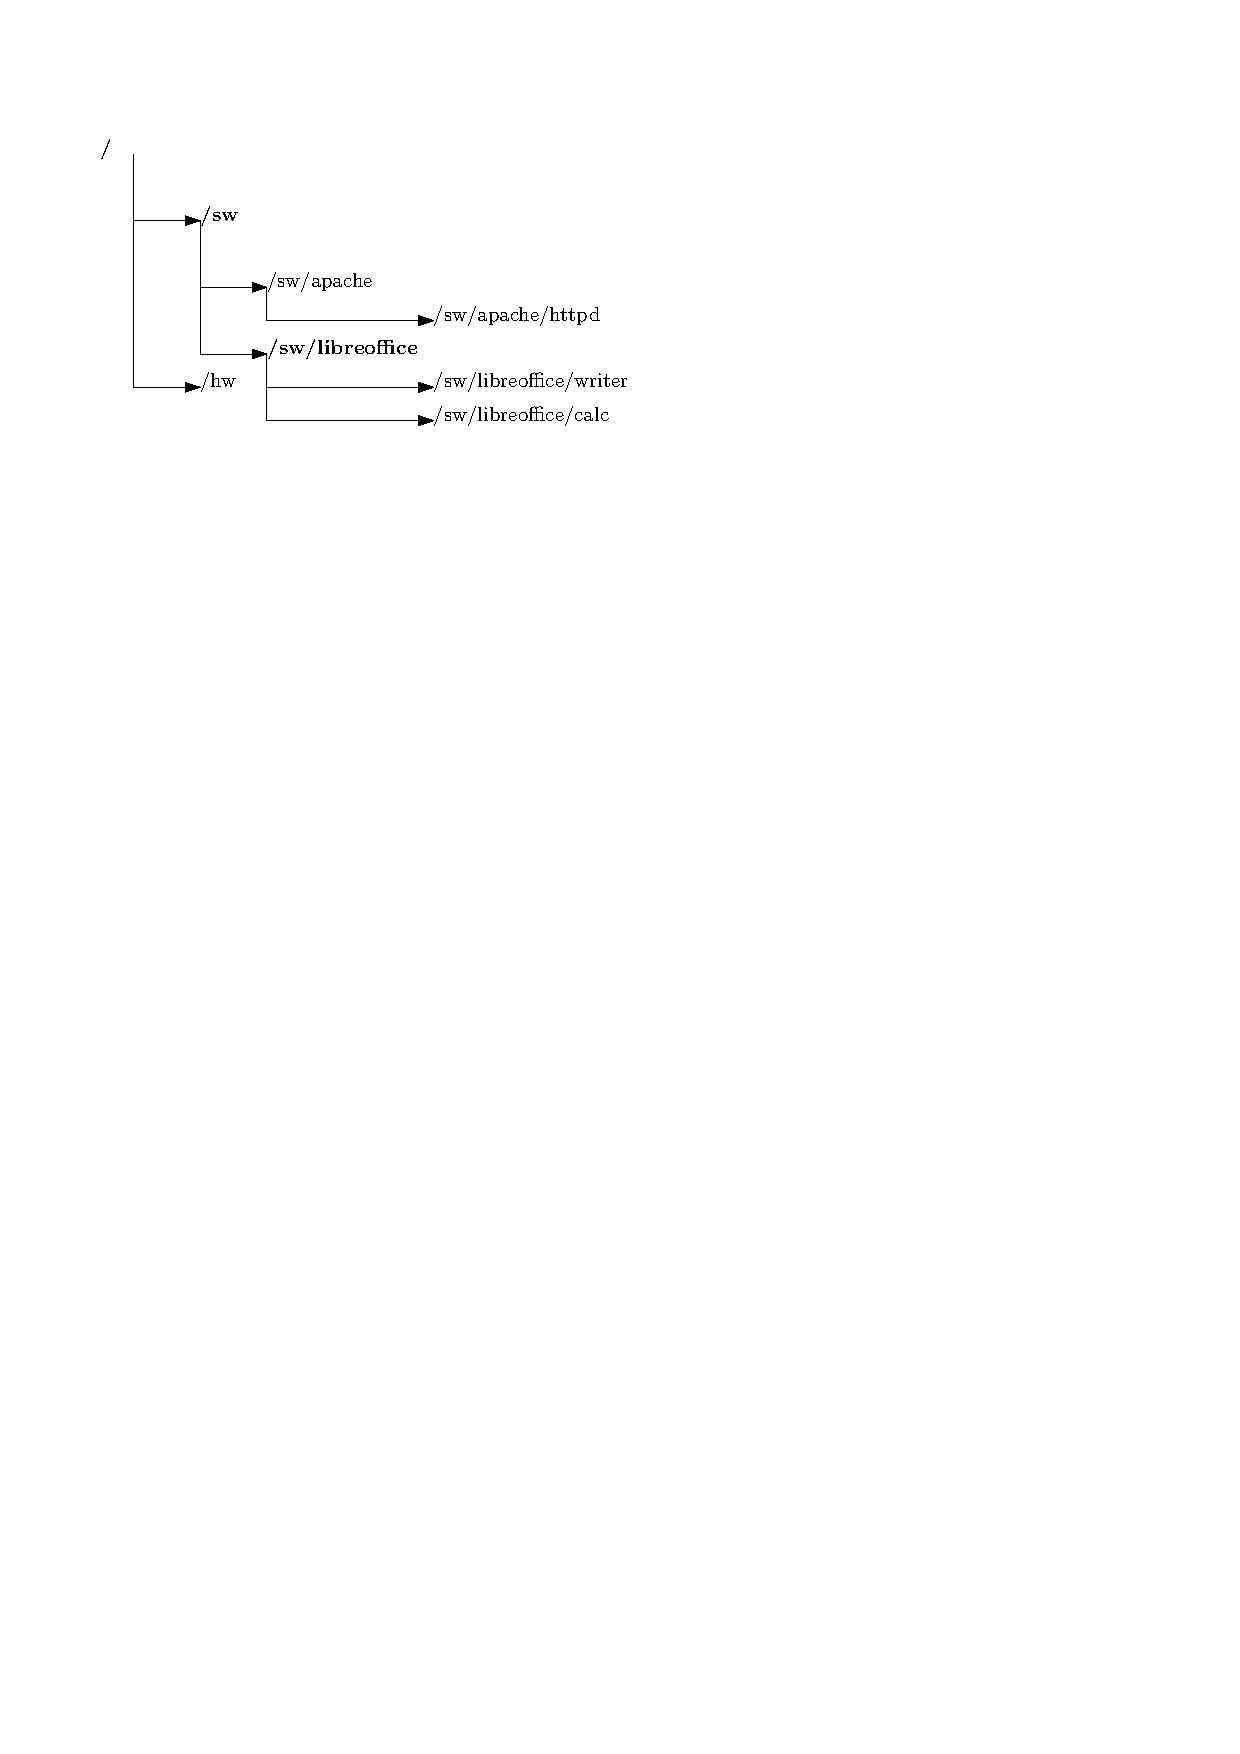
\includegraphics{mounting}
\end{frame}

\begin{frame}
	\frametitle{Plugins}

	Different backends can use different plugins:
	\begin{description}[labelsep=10cm,align=right]
	\item[\texttt{/sw}] in the INI file config.ini
	\item[\texttt{/sw/libreoffice}] in the XML file libreoffice.xml
	\end{description}

	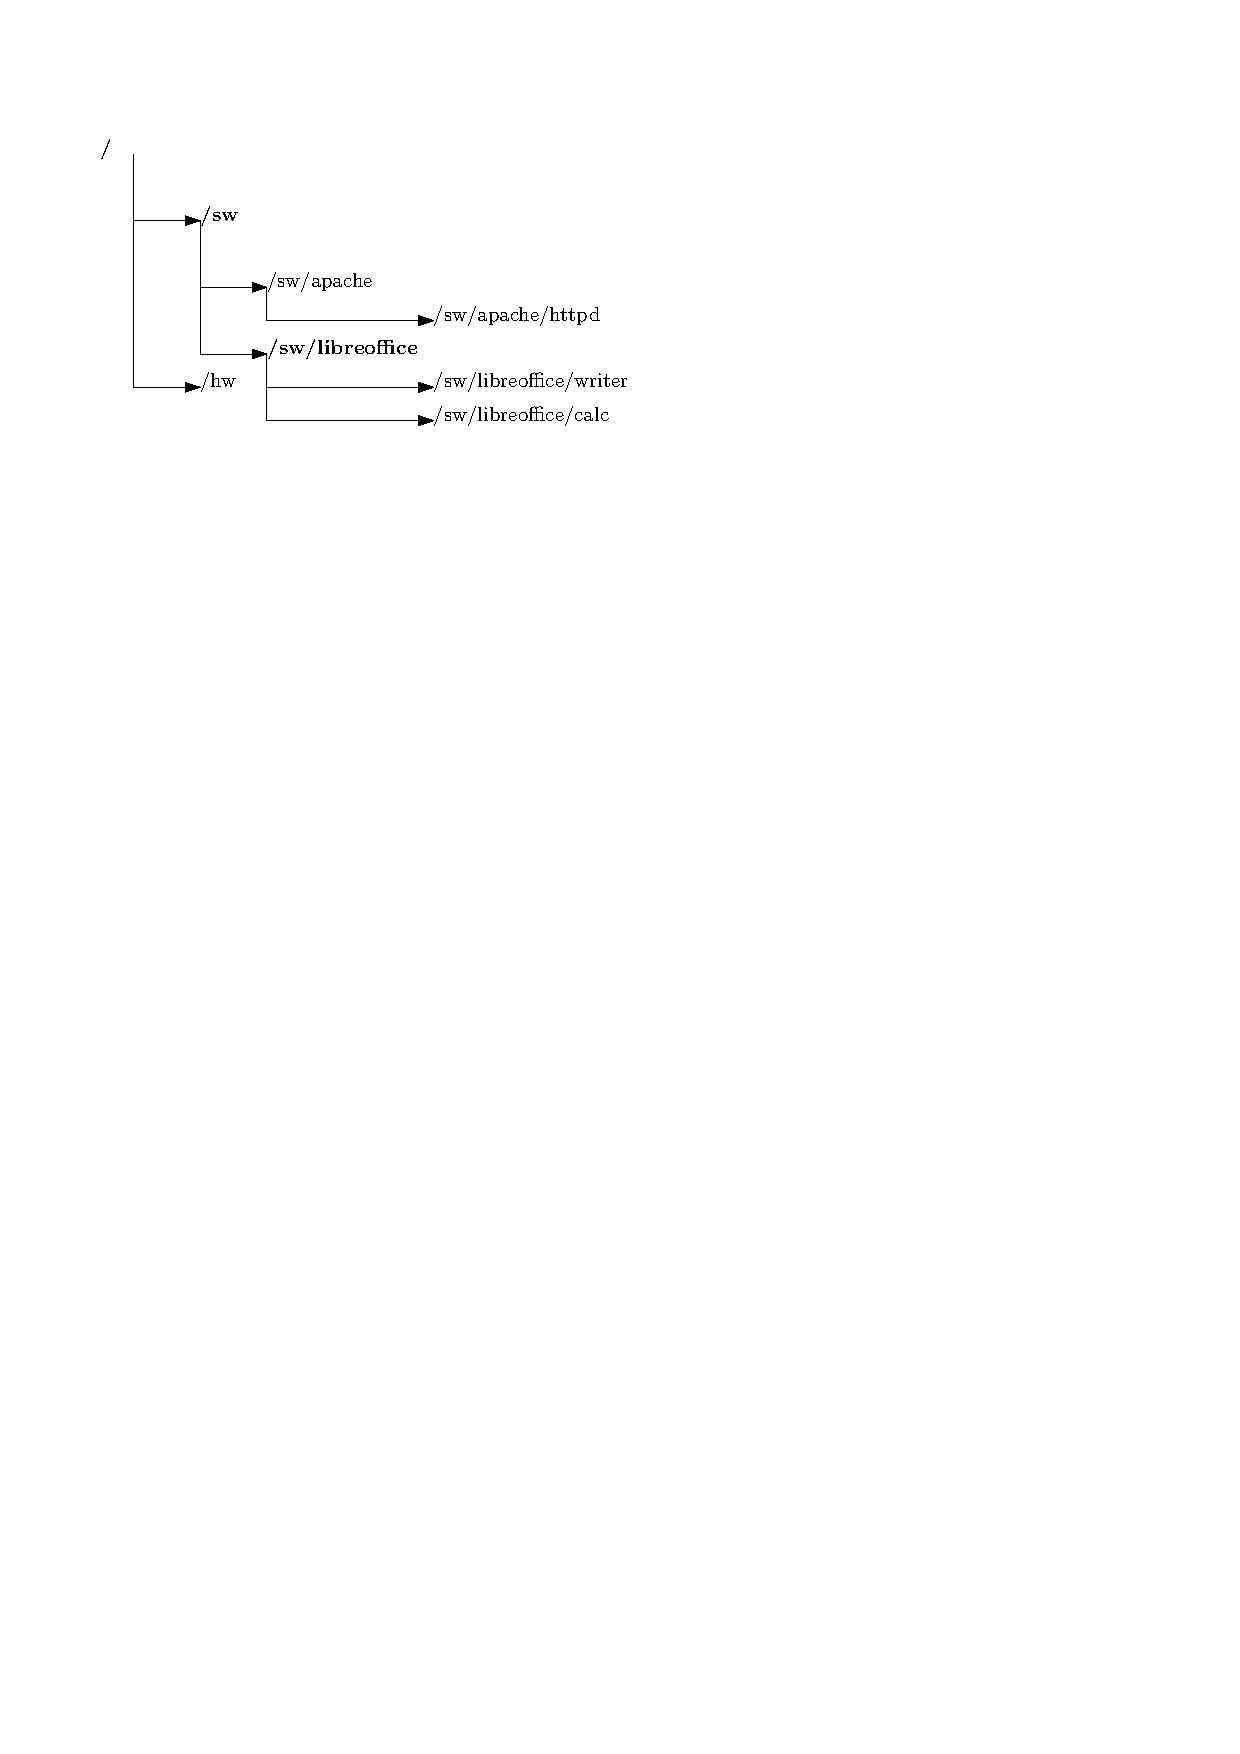
\includegraphics{mounting}
\end{frame}

\begin{assignment}
	\begin{task}
	Explain your neighbor what mounting is.
	\end{task}
\end{assignment}


\subsection{Trend and Outlook}

\begin{frame}
	\frametitle{Trend Firefox}
	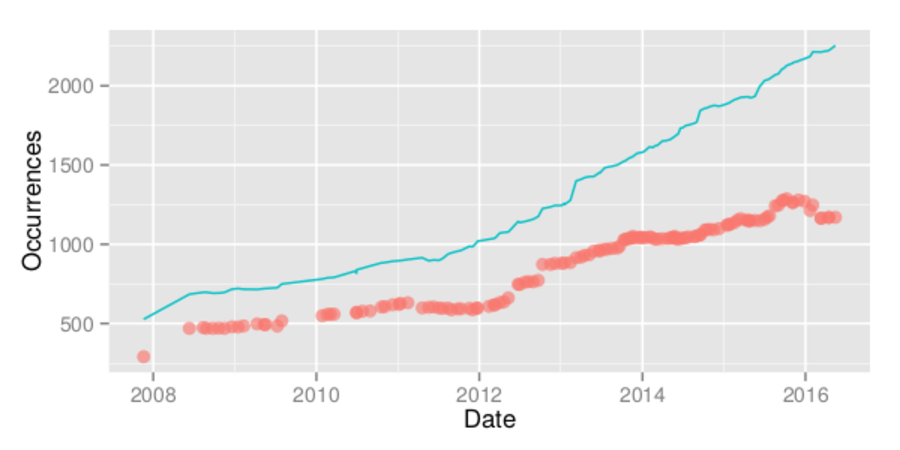
\includegraphics[scale=0.7]{firefox}
\end{frame}

\begin{frame}
	\frametitle{Trend Chromium}
	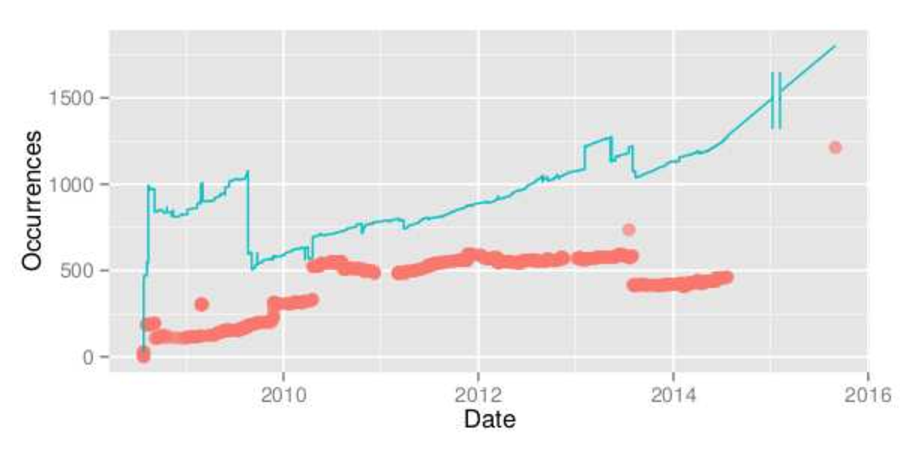
\includegraphics[scale=0.7]{chromium}
\end{frame}

\begin{frame}
	\frametitle{Outlook}
	\begin{itemize}
	\item Environment Variables
	\item Command-line options
	\item Complexity
	\end{itemize}
\end{frame}




%%%%%%%%%%%%%%%%%%%%%%%%%%%%%%%%%%%%%%%%%% 
\nocite{raab2017introducing}

\appendix

\begin{frame}[allowframebreaks]
	\bibliographystyle{plainnat}
	\bibliography{../shared/elektra.bib}
\end{frame}

\end{document}


